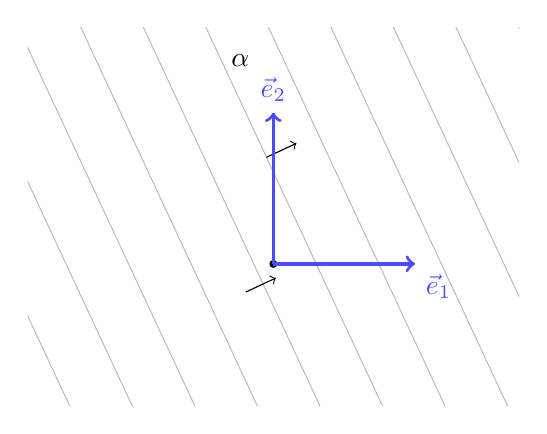
\begin{tikzpicture}[scale=1.2]
  \clip (-2.6,-2.0) rectangle (2.6,2.0);

  % Diagonal level sets for a generic covector alpha
  \begin{scope}[rotate=25]
    \foreach \x in {-4,-3.4,...,4} {
      \draw[gray!55, line width=0.35pt] (\x,-4) -- (\x,4);
    }
    % small direction markers (indicating increasing values)
    \draw[->, black, line width=0.4pt] (-0.6,-0.6) -- (-0.25,-0.6);
    \draw[->, black, line width=0.4pt] (0.2,0.6) -- (0.55,0.6);
  \end{scope}

  % Basis vectors e1, e2
  \fill[black] (0,-0.5) circle (1.2pt);
  \draw[->, very thick, blue!70] (0,-0.5) -- (1.5,-0.5) node[below right] {$\vec{e}_1$};
  \draw[->, very thick, blue!70] (0,-0.5) -- (0,1.1) node[above] {$\vec{e}_2$};

  % labels
  \node at (-0.35,1.65) {$\alpha$};
\end{tikzpicture}
